\documentclass[a4paper,11pt,english]{article}

\usepackage[margin=1.5in,top=1.2in,bottom=1.4in]{geometry}

\usepackage{amsmath}
\usepackage{graphicx}

\usepackage[ngerman]{babel}
\usepackage[utf8]{inputenc}
\usepackage[babel,german=quotes]{csquotes}
\usepackage[hyphens]{url}
\usepackage{listings}
\usepackage{color}
\usepackage{textcomp}
\usepackage[breaklinks]{hyperref}
\usepackage{framed} 
\usepackage[ngerman]{translator}
\usepackage{setspace}


% Sans-Serif-Font
\renewcommand{\familydefault}{\sfdefault}

% kein Einzug in erster Zeile
\setlength{\parindent}{0pt}

% dafür etwas Abstand
\setlength{\parskip}{5pt}

\makeatletter
\DeclareRobustCommand{\em}{%
  \@nomath\em \if b\expandafter\@car\f@series\@nil
  \normalfont \else \bfseries \fi}
\makeatother

\makeatletter
\renewcommand{\maketitle}{
	\begin{center}
		\begin{spacing}{0.8}
		\small
		\@author
		\end{spacing}\large
		{\LARGE\@title}
	\end{center}
\@thanks}
\makeatother

% infobox
\definecolor{boxBG}{rgb}{0.90,0.90,0.96}
\makeatletter\newenvironment{infobox}{%
   \begin{lrbox}{\@tempboxa}\begin{minipage}{\columnwidth}\footnotesize \emph{INFO:} }{\end{minipage}\end{lrbox}%
   \colorbox{boxBG}{\hspace{0pt}\usebox{\@tempboxa}\hspace{0pt}}
}\makeatother

% Additional Options
\definecolor{javared}{rgb}{0.6,0,0} % for strings
\definecolor{javagreen}{rgb}{0.25,0.5,0.35} % comments
\definecolor{javapurple}{rgb}{0.5,0,0.35} % keywords
\definecolor{javadocblue}{rgb}{0.25,0.35,0.75} % javadoc
\definecolor{grey}{rgb}{0.75,0.75,0.75}
\definecolor{darkgrey}{rgb}{0.3,0.3,0.3}
\definecolor{lightgrey}{rgb}{0.95,0.95,0.95}
\definecolor{listingbg}{rgb}{0.90,0.96,0.90}

\lstset{
	language=Python,
	basicstyle=\ttfamily,
	keywordstyle=\color{javapurple}\bfseries,
	stringstyle=\color{javared},
	commentstyle=\color{javagreen},
	morecomment=[s][\color{javadocblue}]{/**}{*/},
	numbers=none, %left
	numberstyle=\color{darkgrey},
	stepnumber=1,
	numbersep=10pt,
	tabsize=4,
	showspaces=false,
	showstringspaces=false,
	breaklines=true,
	breakatwhitespace=false,
	prebreak = \raisebox{0ex}[0ex][0ex]{\ensuremath{\hookleftarrow}},
	frame=l,
	rulecolor=\color{javagreen},
	columns=flexible,
	backgroundcolor=\color{listingbg}
}

\hypersetup{
	pdfborder=0 0 0,
	pdffitwindow=false,    % window fit to page when opened
	pdfstartview={FitH}    % fits the width of the page to the window  
}
\include{glossary}

\begin{document}
	\title{Programmieren lernen mit Python\\1 – Einstieg}
	\author{Chaos Computer Clup Mainz/Wiesbaden e.V.}
	\maketitle
	
	\subsection*{Was ist Python?}
	Python ist eine \emph{Programmiersprache}. Mit ihr kann man Programme schreiben, die der Computer dann versteht und ausführt. Das können kleine Spiele sein, aber auch richtig große Programme, wie zum Beispiel ein Programm um Texte zu schreiben.
	
	\begin{figure}[htbp]
		\centering
		
\includegraphics[width=0.5\textwidth]{img/python-logo.png}
	\end{figure}
	
	\subsection*{Was brauch ich alles?}
	Auf unseren Laptops ist Python schon installiert. Wenn du zuhause mit Python programmieren möchtest, kannst du auf \url{http://python.org/download/} eine Python-Version für dein Betriebssystem herunterladen und installieren. Wir benutzen hier \emph{Python 3} – das heißt, die Versionsnummer der Datei muss mit 3 beginnen, zum Beispiel \enquote{Python 3.2.2}.
	
	Wenn Python auf deinem Rechner installiert ist, kannst du das Programm \emph{IDLE} starten. IDLE ist eine sogenannte \emph{interaktive Entwicklungsumgebung}. Dabei sind Entwicklungsumgebungen dafür da, dass man seine Programme relativ einfach schreiben kann – ein bisschen wie ein Texteditor für Programmcode.
	
	\begin{figure}[htbp]
		\centering
		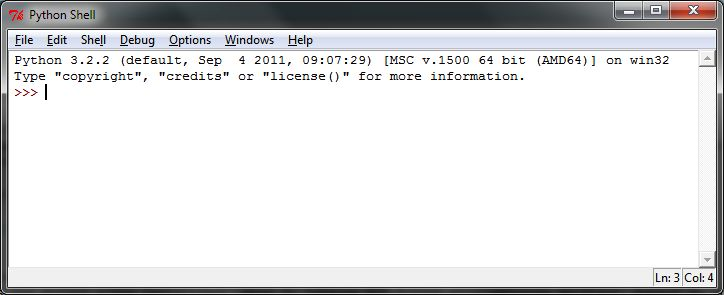
\includegraphics[width=1\textwidth]{img/idle.jpg}
		\caption{IDLE - die interaktive Entwicklungsumgebung für Python}
		\label{IDLE}
	\end{figure}
	
	\subsection*{Ich will Programmieren!}
	Das Fenster, das du vor dir hast, wenn du IDLE öffnest ist die sogenannte \emph{Shell}. Hier kannst du schon einzelne Befehle an den Computer schicken, sodass er die dann ausführt. Tippe zum Beispiel mal \enquote{1+1} in das Fenster und drücke dann ENTER. Was passiert?
	
	\begin{figure}[htbp]
		\centering
		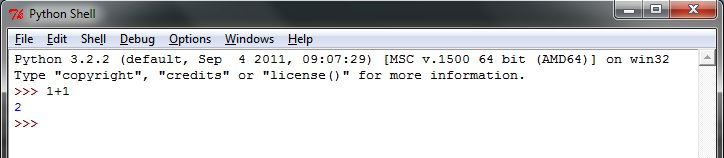
\includegraphics[width=1\textwidth]{img/1plus1.jpg}
		\caption{1+1 - der Befehl zum Ausrechnen}
		\label{1plus1}
	\end{figure}
	
	Du hast dem Computer gerade eine Rechenaufgabe gestellt und er hat sie für dich gelöst. Beim Programmieren werden solche Rechenaufgaben \emph{Ausdrücke} genannt. Dein Ausdruck war noch ziemlich einfach. Aber egal wie kompliziert der Ausdruck ist, der Computer wird immer versuchen, ihn auf einen einzigen Wert runter zu brechen. Das nennen Programmierer auch \enquote{\emph{einen Ausdruck evaluieren}}. 
	
	Probier mit der folgenden Tabelle doch auch mal kompliziertere Ausdrücke aus:
	\begin{table}[htbp]
		\centering
		\normalsize
		\begin{tabular}{|l|l|}
			\hline
				+ & 	addieren (Plus)	\\
			\hline
				- & 	subtrahieren (Minus)\\
			\hline
				* & 	multiplizieren (Mal)\\
			\hline
				/ & 	dividieren (Geteilt)\\
			\hline
		\end{tabular}
	\end{table}
	
	\subsection*{Noch mehr Befehle}
	Die Python-Shell ist natürlich noch viel mehr als ein einfacher Taschenrechner. Hier sind noch mehr Ausdrücke, die du mal ausprobieren kannst. Hättest du die Ergebnisse erwartet? Gibt es auch Ausdrücke, die Python nicht versteht oder nicht ausrechnen kann?
	
	\begin{lstlisting}
>>> 1+2+3+4+5
>>> 1+5*5
>>> (1+6)*5
>>> 1.5-0.5
>>> "Hallo"
>>> "Hallo " + "Welt"
>>> "Hallo " * 3
	\end{lstlisting}
	
\end{document}